\documentclass[tikz,border=10pt]{standalone}
% Shared look for every TikZ diagram. Load with % Shared look for every TikZ diagram. Load with % Shared look for every TikZ diagram. Load with \input{../../tools/tikz-style.tex}
\usepackage[T1]{fontenc}
\usepackage{lmodern}
\renewcommand{\sfdefault}{lmr}  % diagrams use the same serif as the text
\usetikzlibrary{arrows.meta, positioning, shapes.geometric, calc, fit, backgrounds}
\definecolor{cblue}{HTML}{4C78A8}
\definecolor{corange}{HTML}{F58518}
\definecolor{cgreen}{HTML}{54A24B}
\definecolor{cred}{HTML}{E45756}
\definecolor{cpurple}{HTML}{B279A2}
\definecolor{cgrey}{HTML}{6B6B6B}
\tikzset{
  every picture/.style={font=\sffamily, line width=1.2pt},
  box/.style={draw=#1, fill=#1!12, rounded corners=4pt, align=center, inner sep=7pt, minimum height=1.1cm},
  box/.default=cgrey,
  arrow/.style={-{Stealth[length=3mm]}, draw=cgrey, line width=1.4pt},
  title/.style={font=\sffamily\bfseries\Large},
  note/.style={font=\sffamily\small, text=cgrey, align=center},
}
\AtBeginDocument{\hyphenpenalty=10000 \exhyphenpenalty=10000}

\usepackage[T1]{fontenc}
\usepackage{lmodern}
\renewcommand{\sfdefault}{lmr}  % diagrams use the same serif as the text
\usetikzlibrary{arrows.meta, positioning, shapes.geometric, calc, fit, backgrounds}
\definecolor{cblue}{HTML}{4C78A8}
\definecolor{corange}{HTML}{F58518}
\definecolor{cgreen}{HTML}{54A24B}
\definecolor{cred}{HTML}{E45756}
\definecolor{cpurple}{HTML}{B279A2}
\definecolor{cgrey}{HTML}{6B6B6B}
\tikzset{
  every picture/.style={font=\sffamily, line width=1.2pt},
  box/.style={draw=#1, fill=#1!12, rounded corners=4pt, align=center, inner sep=7pt, minimum height=1.1cm},
  box/.default=cgrey,
  arrow/.style={-{Stealth[length=3mm]}, draw=cgrey, line width=1.4pt},
  title/.style={font=\sffamily\bfseries\Large},
  note/.style={font=\sffamily\small, text=cgrey, align=center},
}
\AtBeginDocument{\hyphenpenalty=10000 \exhyphenpenalty=10000}

\usepackage[T1]{fontenc}
\usepackage{lmodern}
\renewcommand{\sfdefault}{lmr}  % diagrams use the same serif as the text
\usetikzlibrary{arrows.meta, positioning, shapes.geometric, calc, fit, backgrounds}
\definecolor{cblue}{HTML}{4C78A8}
\definecolor{corange}{HTML}{F58518}
\definecolor{cgreen}{HTML}{54A24B}
\definecolor{cred}{HTML}{E45756}
\definecolor{cpurple}{HTML}{B279A2}
\definecolor{cgrey}{HTML}{6B6B6B}
\tikzset{
  every picture/.style={font=\sffamily, line width=1.2pt},
  box/.style={draw=#1, fill=#1!12, rounded corners=4pt, align=center, inner sep=7pt, minimum height=1.1cm},
  box/.default=cgrey,
  arrow/.style={-{Stealth[length=3mm]}, draw=cgrey, line width=1.4pt},
  title/.style={font=\sffamily\bfseries\Large},
  note/.style={font=\sffamily\small, text=cgrey, align=center},
}
\AtBeginDocument{\hyphenpenalty=10000 \exhyphenpenalty=10000}

\begin{document}
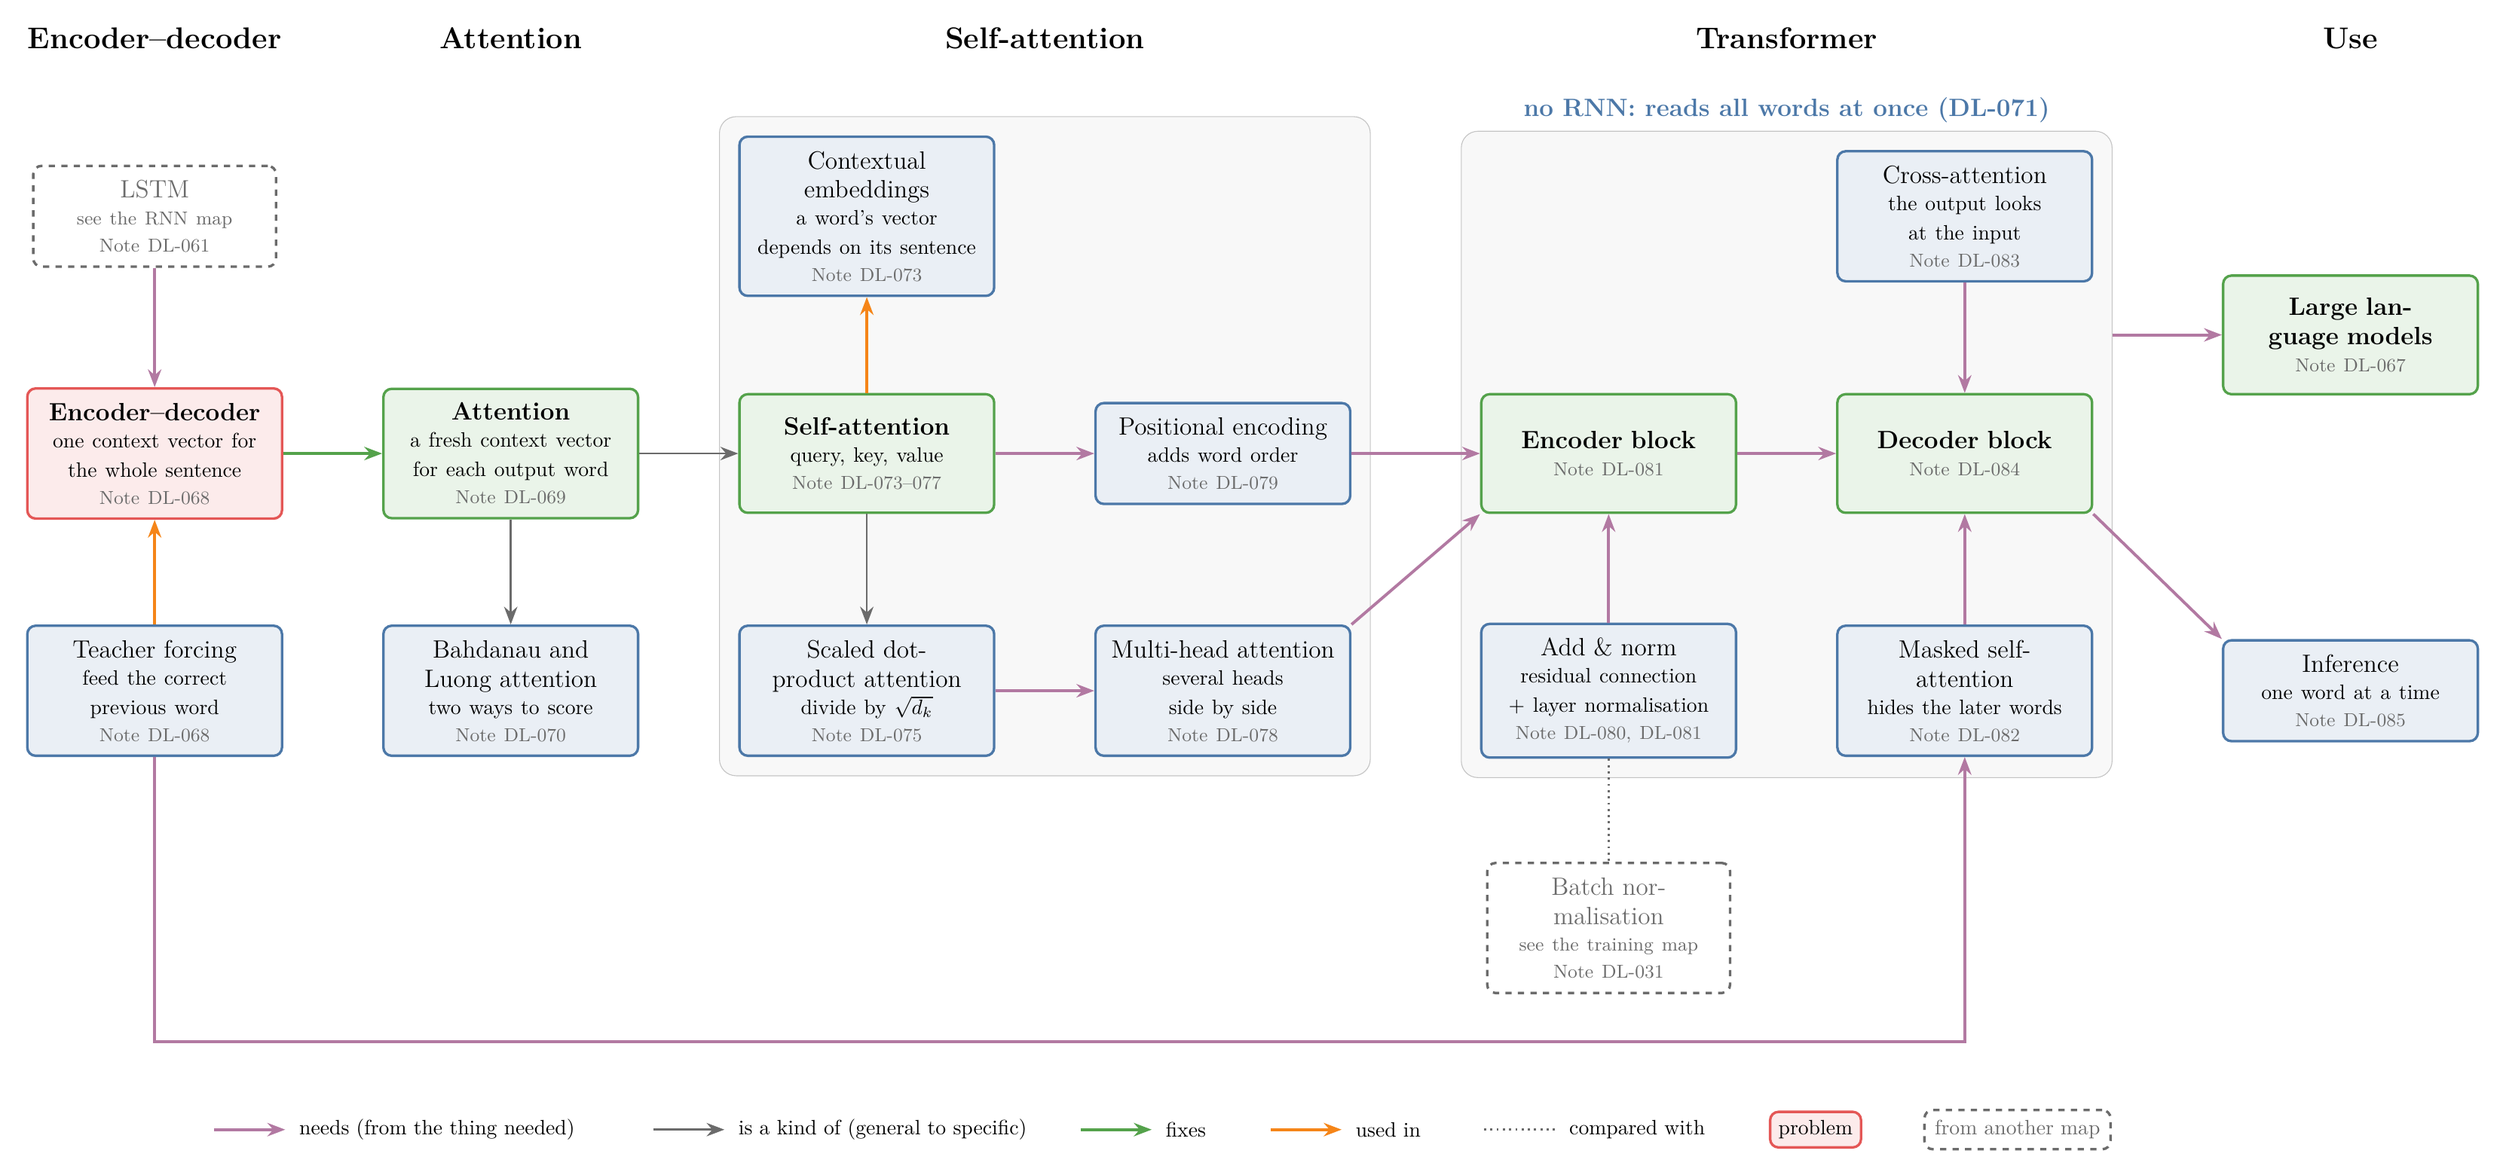
\begin{tikzpicture}[
    every node/.append style={font=\sffamily\large},
    con/.style={box=cblue, text width=3.8cm},
    prob/.style={box=cred, text width=3.8cm},
    prev/.style={draw=cgrey, dashed, rounded corners=4pt, align=center, inner sep=7pt, text=cgrey, text width=3.6cm, minimum height=1.1cm},
    group/.style={draw=cgrey!40, fill=cgrey!5, rounded corners=8pt, inner sep=9pt},
    kind/.style={arrow, draw=cgrey, line width=1pt},
    needs/.style={arrow, draw=cpurple},
    fixes/.style={arrow, draw=cgreen},
    usedin/.style={arrow, draw=corange},
    cmp/.style={draw=cgrey, line width=1pt, dotted},
  ]
  \newcommand{\nt}[1]{\\[-1pt]{\small\color{cgrey}Note #1}}
  \newcommand{\sub}[1]{\\[-1pt]{\normalsize #1}}
  \node[title] at (0,9.4) {Encoder--decoder};
  \node[title] at (6,9.4) {Attention};
  \node[title] at (15,9.4) {Self-attention};
  \node[title] at (27.5,9.4) {Transformer};
  \node[title] at (37,9.4) {Use};

  % encoder-decoder
  \node[prev] (lstm) at (0,6.4) {LSTM\\[-1pt]{\small see the RNN map}\nt{DL-061}};
  \node[prob] (s2s) at (0,2.4) {\textbf{Encoder--decoder}\sub{one context vector for the whole sentence}\nt{DL-068}};
  \node[con] (tf) at (0,-1.6) {Teacher forcing\sub{feed the correct previous word}\nt{DL-068}};
  \draw[needs] (lstm) -- (s2s);
  \draw[usedin] (tf) -- (s2s);

  % attention
  \node[box=cgreen, text width=3.8cm] (att) at (6,2.4) {\textbf{Attention}\sub{a fresh context vector for each output word}\nt{DL-069}};
  \node[con] (bl) at (6,-1.6) {Bahdanau and Luong attention\sub{two ways to score}\nt{DL-070}};
  \draw[fixes] (s2s) -- (att);
  \draw[kind] (att) -- (bl);

  % self-attention
  \node[con] (ctx) at (12,6.4) {Contextual embeddings\sub{a word's vector depends on its sentence}\nt{DL-073}};
  \node[box=cgreen, text width=3.8cm, minimum height=2.0cm] (self) at (12,2.4) {\textbf{Self-attention}\sub{query, key, value}\nt{DL-073--077}};
  \node[con] (sdp) at (12,-1.6) {Scaled dot-product attention\sub{divide by $\sqrt{d_k}$}\nt{DL-075}};
  \node[con] (pos) at (18,2.4) {Positional encoding\sub{adds word order}\nt{DL-079}};
  \node[con] (mha) at (18,-1.6) {Multi-head attention\sub{several heads side by side}\nt{DL-078}};
  \begin{scope}[on background layer]
    \node[group, fit=(ctx) (self) (sdp) (pos) (mha)] (gs) {};
  \end{scope}
  \draw[kind] (att) -- (self);
  \draw[usedin] (self) -- (ctx);
  \draw[kind] (self) -- (sdp);
  \draw[needs] (self) -- (pos);
  \draw[needs] (sdp) -- (mha);

  % transformer: encoder and decoder blocks
  \node[box=cgreen, text width=3.8cm, minimum height=2.0cm] (enc) at (24.5,2.4) {\textbf{Encoder block}\nt{DL-081}};
  \node[con] (an) at (24.5,-1.6) {Add \& norm\sub{residual connection + layer normalisation}\nt{DL-080, DL-081}};
  \node[box=cgreen, text width=3.8cm, minimum height=2.0cm] (dec) at (30.5,2.4) {\textbf{Decoder block}\nt{DL-084}};
  \node[con] (cross) at (30.5,6.4) {Cross-attention\sub{the output looks at the input}\nt{DL-083}};
  \node[con] (mask) at (30.5,-1.6) {Masked self-attention\sub{hides the later words}\nt{DL-082}};
  \node[prev] (bn) at (24.5,-5.6) {Batch normalisation\\[-1pt]{\small see the training map}\nt{DL-031}};
  \begin{scope}[on background layer]
    \node[group, fit=(enc) (an) (dec) (cross) (mask)] (gt) {};
  \end{scope}
  \node[font=\sffamily\bfseries\large, text=cblue, anchor=south] at (gt.north) {no RNN: reads all words at once (DL-071)};
  \draw[needs] (pos) -- (enc);
  \draw[needs] (mha.north east) -- (enc.south west);
  \draw[needs] (an) -- (enc);
  \draw[cmp] (an) -- (bn);
  \draw[needs] (enc) -- (dec);
  \draw[needs] (cross) -- (dec);
  \draw[needs] (mask) -- (dec);
  \draw[needs] (tf.south) -- ++(0,-4.8) -| (mask.south);

  % use
  \node[box=cgreen, text width=3.8cm, minimum height=2.0cm] (llm) at (37,4.4) {\textbf{Large language models}\nt{DL-067}};
  \node[con] (inf) at (37,-1.6) {Inference\sub{one word at a time}\nt{DL-085}};
  \draw[needs] (gt.east |- llm.west) -- (llm.west);
  \draw[needs] (dec.south east) -- (inf.north west);

  % legend
  \begin{scope}[shift={(1.0,-9.0)}, every node/.style={font=\sffamily, anchor=west}]
    \draw[needs] (0,0) -- (1.2,0);      \node at (1.3,0) {needs (from the thing needed)};
    \draw[kind] (7.4,0) -- (8.6,0);     \node at (8.7,0) {is a kind of (general to specific)};
    \draw[fixes] (14.6,0) -- (15.8,0);  \node at (15.9,0) {fixes};
    \draw[usedin] (17.8,0) -- (19.0,0); \node at (19.1,0) {used in};
    \draw[cmp] (21.4,0) -- (22.6,0);    \node at (22.7,0) {compared with};
    \node[box=cred, minimum height=0.6cm, inner sep=4pt, anchor=west] at (26.2,0) {problem};
    \node[draw=cgrey, dashed, rounded corners=4pt, inner sep=5pt, text=cgrey, anchor=west] at (28.8,0) {from another map};
  \end{scope}
\end{tikzpicture}
\end{document}
